\section{TCP主动打开-客户}
\label{sec:tcp_connect_client}

    \subsection{基本流程}
    \label{subsec:tcp_connect_flow}
        客户端的主动打开是通过connect系统调用等一系列操作来完成的,这一系统调用最终会调用传输层的\mintinline{c}{tcp_v4_connect}函数。基本就是客户端发送SYN段,接收SYN+ACK段,最后再次发送ACK段给服务器。

    \subsection{第一次握手:构造并发送SYN包}
    \label{subsec:tcp_connect_syn}

        \subsubsection{基本调用关系}

                \begin{figure}[htb]        
                    \centering
                    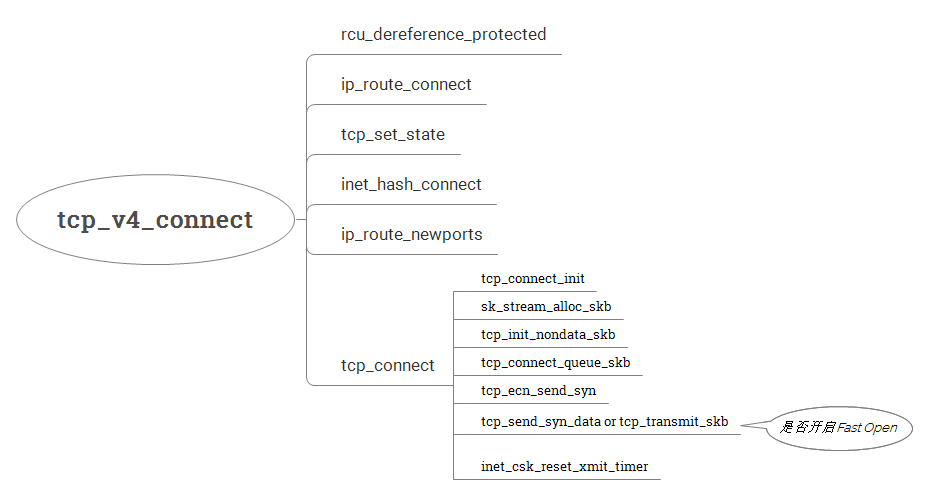
\includegraphics[width=\textwidth]  {images/Client:Send SYN.png}
					\caption{Client:Send SYN}
					\label{Client:Send SYN}
                \end{figure}            
        \subsubsection{\mintinline{C}{tcp_v4_connect}}
        	\label{Client:tcp_v4_connect}

            \mintinline{c}{tcp_v4_connect}的主要作用是进行一系列的判断,初始化传输控制块
            并调用相关函数发送SYN包。
\begin{minted}[linenos]{c}
/*
Location:

    net/ipv4/tcp_ipv4.c

Function:

    这个函数会初始化一个的连接。

Parameters:

    sk:传输控制块
    uaddr:通用地址结构,包含所属协议字段和相应的地址字段。
    addr_len :目的地址长度
*/
int tcp_v4_connect(struct sock *sk, struct sockaddr *uaddr, int addr_len)
{
        /*
            sockaddr_in结构体用于描述一个Internet (IP) 套接字的地址     
        */
        struct sockaddr_in *usin = (struct sockaddr_in *)uaddr; 
        struct inet_sock *inet = inet_sk(sk);
        struct tcp_sock *tp = tcp_sk(sk);
		/*
			网络协议主要使用大端存储,
			be16 means 16 bits stored with big-endian
			be32,the same.
		*/
        __be16 orig_sport, orig_dport;
        __be32 daddr, nexthop;                  
        struct flowi4 *fl4;
        struct rtable *rt;
        int err;
        struct ip_options_rcu *inet_opt;

        /* 检验目的地址长度是否有效 */
        if (addr_len < sizeof(struct sockaddr_in))
                return -EINVAL;                 //Invalid argument 错误码为22

        /* 检验协议族是否正确 */
        if (usin->sin_family != AF_INET)  //IPV4地址域
                return -EAFNOSUPPORT;     //Address family not supported by protocol

        /* 将下一跳地址和目的地址暂时设置为用户传入的IP地址 */
        nexthop = daddr = usin->sin_addr.s_addr;
        inet_opt = rcu_dereference_protected(inet->inet_opt,
                                             sock_owned_by_user(sk));
        /* 如果选择源地址路由,则将下一跳地址设置为IP选项中的faddr-first hop address*/
        if (inet_opt && inet_opt->opt.srr) {
                if (!daddr)
                        return -EINVAL;
                nexthop = inet_opt->opt.faddr;
        }
\end{minted}

			上面	rcu\_dereference\_protected函数使用了RCU锁,RCU锁的基本介绍参见\ref{Appendix:RCU}.

            源地址路由是一种特殊的路由策略。一般路由都是通过目的地址来进行的。而有时也需要
            通过源地址来进行路由,例如在有多个网卡等情况下,可以根据源地址来决定走哪个网卡等等。

\begin{minted}[linenos]{c}
        orig_sport = inet->inet_sport;
        orig_dport = usin->sin_port;
        fl4 = &inet->cork.fl.u.ip4;     //对应于ipv4的流
        /* 获取目标的路由缓存项,如果路由查找命中,则生成一个相应的路由缓存项,
			这个缓存项不但可以用于当前待发送的SYN段,而且对后续的所有数据包都
			可以起到一个加速路由查找的作用。
		*/
        rt = ip_route_connect(fl4, nexthop, inet->inet_saddr,
                              RT_CONN_FLAGS(sk), sk->sk_bound_dev_if,
                              IPPROTO_TCP,
                              orig_sport, orig_dport, sk);
        /*判断指针是否有效*/        
        if (IS_ERR(rt)) {
                err = PTR_ERR(rt);
                if (err == -ENETUNREACH)    //Network is unreachable
                        IP_INC_STATS(sock_net(sk), IPSTATS_MIB_OUTNOROUTES);
                return err;
        }
\end{minted}

		对于函数IS\_ERR、PTR\_ERR的具体介绍,请参见\ref{Appendix:ERR}.

\begin{minted}[linenos]{C}
        /*TCP不能使用类型为组播或多播的路由缓存项*/
        if (rt->rt_flags & (RTCF_MULTICAST | RTCF_BROADCAST)) {
                ip_rt_put(rt);
                return -ENETUNREACH;        //Network is unreachable
        }

        /* 如果IP选项为空或者没有开启源路由功能,则采用查找到的缓存项 */
        if (!inet_opt || !inet_opt->opt.srr)
                daddr = fl4->daddr;

        /* 如果没有设置源地址,则设置为缓存项中的源地址 */
        if (!inet->inet_saddr)
                inet->inet_saddr = fl4->saddr;
        sk_rcv_saddr_set(sk, inet->inet_saddr);

        /* 
			如果该传输控制块的时间戳已被使用过,则重置各状态 
            rx_opt:  tcp_options_received
        */
        if (tp->rx_opt.ts_recent_stamp && inet->inet_daddr != daddr) {
                /* Reset inherited state */
                /*下一个待发送的TCP段中的时间戳回显值*/
                tp->rx_opt.ts_recent       = 0;     
                /*从接收到的段中取出时间戳*/
                tp->rx_opt.ts_recent_stamp = 0;
                /*What does it means repair*/       
                if (likely(!tp->repair))
                        tp->write_seq      = 0;
        }

        /*  
			在启用了tw_recycle:time wait recycle的情况下,重设时间戳 
            它用来快速回收TIME_WAIT连接.
        */
        if (tcp_death_row.sysctl_tw_recycle &&
            !tp->rx_opt.ts_recent_stamp && fl4->daddr == daddr)
                tcp_fetch_timewait_stamp(sk, &rt->dst);

        /* 设置传输控制块 */
        inet->inet_dport = usin->sin_port;
        sk_daddr_set(sk, daddr);

        inet_csk(sk)->icsk_ext_hdr_len = 0;
        if (inet_opt)
                inet_csk(sk)->icsk_ext_hdr_len = inet_opt->opt.optlen;

        /* 设置MSS大小 */
        tp->rx_opt.mss_clamp = TCP_MSS_DEFAULT;

        /* Socket identity is still unknown (sport may be zero).
         * However we set state to SYN-SENT and not releasing socket
         * lock select source port, enter ourselves into the hash tables and
         * complete initialization after this.
         */
        /* 将TCP的状态设置为SYN_SENT */
        tcp_set_state(sk, TCP_SYN_SENT);
        err = inet_hash_connect(&tcp_death_row, sk);
        if (err)
                goto failure;

        sk_set_txhash(sk);

        /*
			如果源端口或者目的端口发生改变,则需要重新查找路由,
			并用新的路由缓存项更新sk中保存的路由缓存项。
		*/
        rt = ip_route_newports(fl4, rt, orig_sport, orig_dport,
                               inet->inet_sport, inet->inet_dport, sk);
        if (IS_ERR(rt)) {
                err = PTR_ERR(rt);
                rt = NULL;
                goto failure;
        }
        /* 将目的地址提交到套接字  */
        sk->sk_gso_type = SKB_GSO_TCPV4;
        sk_setup_caps(sk, &rt->dst);

        /*  
			如果没有设置序号,则计算初始序号 
            序号与双方的地址与端口号有关系
        */
        if (!tp->write_seq && likely(!tp->repair))
                tp->write_seq = secure_tcp_sequence_number(inet->inet_saddr,
                                                           inet->inet_daddr,
                                                           inet->inet_sport,
                                                           usin->sin_port);
                                                           
        /*  
			计算IP首部的id域的值 
            全局变量jiffies用来记录自系统启动以来产生的节拍的总数       
        */
        inet->inet_id = tp->write_seq ^ jiffies;

        /* 调用tcp_connect构造并发送SYN包*/
        err = tcp_connect(sk);

        rt = NULL;
        if (err)
                goto failure;

        return 0;
\end{minted}

            总结起来,\mintinline{c}{tcp_v4_connect}是在根据用户提供的目的地址,
            设置好了传输控制块,为传输做好准备。如果在这一过程中出现错误,则会跳到
            错误处理代码。
\begin{minted}[linenos]{c}
failure:
        /* 将状态设定为TCP_CLOSE,释放端口,并返回错误值。
         */
        tcp_set_state(sk, TCP_CLOSE);
        ip_rt_put(rt);
        sk->sk_route_caps = 0;
        inet->inet_dport = 0;
        return err;
\end{minted}

        \subsubsection{\mintinline{C}{tcp_connect}}
			\label{Client:tcp_connect}
            上面的\mintinline{c}{tcp_v4_connect}会进行一系列的判断,之后真正构造SYN包的部分
            被放在了\mintinline{c}{tcp_connect}中。接下来,我们来分析这个函数。

\begin{minted}[linenos]{c}
/* 
Location:

    net/ipv4/tcp_output.c

Function:

    该函数用于构造并发送SYN包。

Parameter:

    sk:传输控制块。

 */
int tcp_connect(struct sock *sk)
{
        struct tcp_sock *tp = tcp_sk(sk);
        struct sk_buff *buff;
        int err;

        /* 初始化tcp连接 */
        tcp_connect_init(sk);
\end{minted}

		关于tcp\_connect\_init更多的内容,请参见\ref{TCPInitialize:tcp_connect_init}。
\begin{minted}[linenos]{C}
        if (unlikely(tp->repair)) {             //what does it mean repair?
                /* 如果repair位被置1,那么结束TCP连接 */
                tcp_finish_connect(sk, NULL);
                return 0;
        }

        /* 分配一个sk_buff */
        buff = sk_stream_alloc_skb(sk, 0, sk->sk_allocation, true);
        if (unlikely(!buff))
                return -ENOBUFS;                //No buffer space available

        /* 初始化skb,并自增write_seq的值 */
        tcp_init_nondata_skb(buff, tp->write_seq++, TCPHDR_SYN);
\end{minted}
	       
		关于tcp\_init\_nondata\_skb更多的内容,请参见\ref{TCPInitialize:tcp_init_nondata_skb}。

\begin{minted}[linenos]{C} 
		/* 设置时间戳 */
        tp->retrans_stamp = tcp_time_stamp;
        /* 将当前的sk_buff添加到发送队列中 */
        tcp_connect_queue_skb(sk, buff);
        /* 
			ECN (Explicit Congestion Notification,)
			支持显式拥塞控制
        */
        tcp_ecn_send_syn(sk, buff);         //what does this function do?

        /* 
			发送SYN包,这里同时还考虑了Fast Open的情况,意思就是
			可以在连接建立的时候同时发数据。
		*/
        err = tp->fastopen_req ? tcp_send_syn_data(sk, buff) :
              tcp_transmit_skb(sk, buff, 1, sk->sk_allocation);
        if (err == -ECONNREFUSED)           /*Connection refused*/
                return err;

        /* We change tp->snd_nxt after the tcp_transmit_skb() call
         * in order to make this packet get counted in tcpOutSegs.
         */
        tp->snd_nxt = tp->write_seq;     //send next 下一个待发送字节的序列号
        /*pushed_seq means Last pushed seq, required to talk to windows???*/        
        tp->pushed_seq = tp->write_seq;
        TCP_INC_STATS(sock_net(sk), TCP_MIB_ACTIVEOPENS);

        /* 设定超时重传定时器 */
        inet_csk_reset_xmit_timer(sk, ICSK_TIME_RETRANS,
                                  inet_csk(sk)->icsk_rto, TCP_RTO_MAX);
        return 0;
}
\end{minted}

\subsection{第二次握手:接收SYN+ACK包}
\label{Client:Recv SYN+ACK}

    \subsubsection{基本调用关系}

                \begin{figure}[htb]        
                    \centering
                    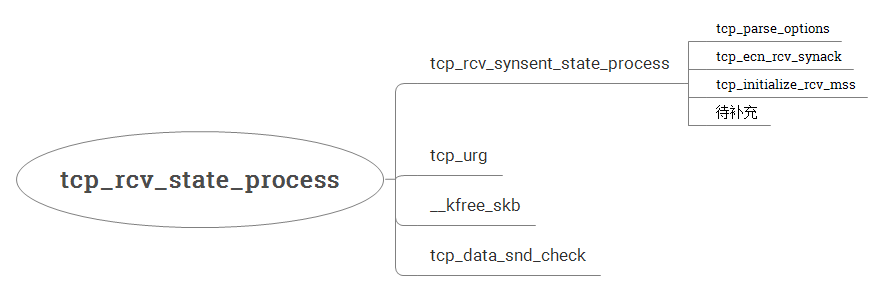
\includegraphics[width=\textwidth]  {images/Client:Receive SYN +ACK.png}
					\caption{Client:Receive SYN+ACK}
					\label{Client:Receive SYN+ACK}
                \end{figure} 

    \subsubsection{\mintinline{c}{tcp_rcv_state_process}}
		\label{SYN+ACK:tcp_rcv_state_process}
        \mintinline{c}{tcp_rcv_state_process}实现了TCP状态机相对核心的一个部分。
        该函数可以处理除ESTABLISHED和TIME\_WAIT状态以外的情况下的接收过程。
        这里,我们仅关心主动连接情况下的处理。在\ref{Client:tcp_v4_connect}中,我们
        分析源码时得出,客户端发送SYN包后,会将状态机设置为\mintinline{c}{TCP_SYN_SENT}状态。
        因此,我们仅在这里分析该状态下的代码。.

\begin{minted}[linenos]{c}
/*
Location:

    net/ipv4/tcp_input.c

Function:

    This function implements the receiving procedure of RFC 793 for
    all states except ESTABLISHED and TIME_WAIT.
    It's called from both tcp_v4_rcv and tcp_v6_rcv and should be
    address independent.

Paramater:

    sk:传输控制块。
    skb:缓存块。
*/
int tcp_rcv_state_process(struct sock *sk, struct sk_buff *skb)
{
        struct tcp_sock *tp = tcp_sk(sk);
        struct inet_connection_sock *icsk = inet_csk(sk);
        const struct tcphdr *th = tcp_hdr(skb);
        struct request_sock *req;
        int queued = 0;
        bool acceptable;

        /*标识接收到的TCP段不存在TCP时间戳选项??why*/
        tp->rx_opt.saw_tstamp = 0;

        switch (sk->sk_state) {
            case TCP_CLOSE:
                    /* CLOSE状态的处理代码 */

            case TCP_LISTEN:
                    /* LISTEN状态的处理代码 */

            case TCP_SYN_SENT:
                    /* 处理接收到的数据段 */
                    queued = tcp_rcv_synsent_state_process(sk, skb, th);
                    if (queued >= 0)
                            return queued;

                    /* 处理紧急数据并检测是否有数据需要发送 */
                    tcp_urg(sk, skb, th);
					/*释放缓存*/
                    __kfree_skb(skb);
                    tcp_data_snd_check(sk);
                    return 0;
            }

        /* 处理其他情况的代码 */
}
\end{minted}

	关于tcp\_urg的详细内容,请参见\ref{TCPUrgent:tcp_urg}.

    \subsubsection{\mintinline{c}{tcp_rcv_synsent_state_process}}
		\label{SYN+ACK:tcp_rcv_synsent_state_process}
        具体的处理代码在\mintinline{c}{tcp_rcv_synsent_state_process}中,通过
        命名就可以看出,该函数是专门用于处理SYN\_SENT状态下收到数据的情况。

\begin{minted}[linenos]{c}
/*
Location:

    net/ipv4/tcp_input.c

Function:

    处理syn已经发送的状态。

Parameter:

    sk:传输控制块
    skb:缓存
    th:tcp报文的头部

*/
static int tcp_rcv_synsent_state_process(struct sock *sk, struct sk_buff *skb,
                                         const struct tcphdr *th)
{
        struct inet_connection_sock *icsk = inet_csk(sk);
        struct tcp_sock *tp = tcp_sk(sk);
        struct tcp_fastopen_cookie foc = { .len = -1 };
        int saved_clamp = tp->rx_opt.mss_clamp;

        /* 解析TCP选项,并保存在传输控制块中 */
        tcp_parse_options(skb, &tp->rx_opt, 0, &foc);
        /*
            rcv_tsecr 保存最近一次接收到对端的TCP段的时间
            戳选项中的时间戳回显应答。???

            tsoffset means timestamp offset
        */
        if (tp->rx_opt.saw_tstamp && tp->rx_opt.rcv_tsecr)
                tp->rx_opt.rcv_tsecr -= tp->tsoffset;
\end{minted}

		关于tcp\_parse\_options的更多的内容,请参见\ref{TCPOptions:tcp_parse_options}。

		接下来的部分,就是按照TCP协议的标准来实现相应的行为。注释中出现的RFC793即是描述TCP协议
		的RFC原文中的文本。
\begin{minted}[linenos]{c}
        if (th->ack) {
                /* rfc793:
                 * "If the state is SYN-SENT then
                 *    first check the ACK bit
                 *      If the ACK bit is set
                 *        If SEG.ACK =< ISS, or SEG.ACK > SND.NXT, send
                 *        a reset (unless the RST bit is set, if so drop
                 *        the segment and return)"
                 * ISS代表初始发送序号(Initial Send Sequence number)
                    snd_una 在输出的段中,最早一个未被确认段的序号
                 */
                if (!after(TCP_SKB_CB(skb)->ack_seq, tp->snd_una) ||
                    after(TCP_SKB_CB(skb)->ack_seq, tp->snd_nxt))
                        goto reset_and_undo;
				/*必须在对应的时间内*/
                if (tp->rx_opt.saw_tstamp && tp->rx_opt.rcv_tsecr &&
                    !between(tp->rx_opt.rcv_tsecr, tp->retrans_stamp,
                             tcp_time_stamp)) {
                        NET_INC_STATS_BH(sock_net(sk), LINUX_MIB_PAWSACTIVEREJECTED);
                        goto reset_and_undo;
                }
\end{minted}
上面的一段根据RFC在判断ACK的值是否在初始发送序号和下一个序号之间,如果不在,则发送一个重置。
\begin{minted}[linenos]{c}
                /* 此时,ACK已经被接受了
                 *
                 * "If the RST bit is set
                 *    If the ACK was acceptable then signal the user "error:
                 *    connection reset", drop the segment, enter CLOSED state,
                 *    delete TCB, and return."
                 */

                if (th->rst) {
                        tcp_reset(sk);
                        goto discard;
                }
\end{minted}
接下来,判断了收到的包的RST位,如果设置了RST,则丢弃该分组,并进入CLOSED状态。
\begin{minted}[linenos]{c}
                /* rfc793:
                 *   "fifth, if neither of the SYN or RST bits is set then
                 *    drop the segment and return."
                 *
                 *    See note below!
                 *                                        --ANK(990513)
                 */
                if (!th->syn)
                        goto discard_and_undo;
\end{minted}
之后,根据RFC的说法,如果既没有设置SYN位,也没有设置RST位,那么就将分组丢弃掉。
前面已经判断了RST位了,因此,这里判断一下SYN位。

接下来就准备进入到ESTABLISHED状态了。
\begin{minted}[linenos]{c}
                /* rfc793:
                 *   "If the SYN bit is on ...
                 *    are acceptable then ...
                 *    (our SYN has been ACKed), change the connection
                 *    state to ESTABLISHED..."
                 */

                tcp_ecn_rcv_synack(tp, th);

                /* 初始化与窗口有关的参数 */
                tcp_init_wl(tp, TCP_SKB_CB(skb)->seq);
                tcp_ack(sk, skb, FLAG_SLOWPATH);

                /* Ok.. it's good. Set up sequence numbers and
                 * move to established.
                 */
                tp->rcv_nxt = TCP_SKB_CB(skb)->seq + 1;
                tp->rcv_wup = TCP_SKB_CB(skb)->seq + 1;
\end{minted}
对于SYN和SYN/ACK段是不进行窗口放大的。关于RFC1323窗口放大相关的内容,我们在
\ref{subsec:rfc1323}中进行了详细讨论。接下来手动设定了窗口缩放相关的参数,
使得缩放不生效。
\begin{minted}[linenos]{c}
                /* RFC1323: The window in SYN & SYN/ACK segments is
                 * never scaled.
                 */
                tp->snd_wnd = ntohs(th->window);    //network to host short int

                /* wscale_ok 标志接收方是否支持窗口扩大因子
                   window_clamp 滑动窗口最大值
                */                
                if (!tp->rx_opt.wscale_ok) {
                        tp->rx_opt.snd_wscale = tp->rx_opt.rcv_wscale = 0;
                        tp->window_clamp = min(tp->window_clamp, 65535U);
                }
\end{minted}
根据时间戳选项,设定相关字段及TCP头部长度。
\begin{minted}[linenos]{c}
                if (tp->rx_opt.saw_tstamp) {
                        tp->rx_opt.tstamp_ok= 1;
                        tp->tcp_header_len =
                                sizeof(struct tcphdr) + TCPOLEN_TSTAMP_ALIGNED;
                        tp->advmss -= TCPOLEN_TSTAMP_ALIGNED;
                        tcp_store_ts_recent(tp);
                } else {
                        tp->tcp_header_len = sizeof(struct tcphdr);
                }
\end{minted}
之后会根据设定开启FACK机制。FACK是在SACK机制上发展来的。SACK用于准确地获知哪些包丢失了
需要重传。开启SACK后,可以让发送端只重传丢失的包。而当重传的包比较多时,会进一步导致网络
繁忙,FASK用来做重传过程中的拥塞控制。
\begin{minted}[linenos]{c}
                if (tcp_is_sack(tp) && sysctl_tcp_fack) //sysctl: system control
                        tcp_enable_fack(tp);
\end{minted}
最后初始化MTU、MSS等参数并完成TCP连接过程。
\begin{minted}[linenos]{c}
                tcp_mtup_init(sk);
                tcp_sync_mss(sk, icsk->icsk_pmtu_cookie);
                tcp_initialize_rcv_mss(sk);

                /* Remember, tcp_poll() does not lock socket!
                 * Change state from SYN-SENT only after copied_seq
                 * is initialized. */
                tp->copied_seq = tp->rcv_nxt;

                smp_mb();
                tcp_finish_connect(sk, skb);
\end{minted}
此后,开始处理一些特殊情况。Fast Open启用的情况下,SYN包也会带有数据。这里调用
\mintinline{c}{tcp_rcv_fastopen_synack}函数处理SYN包附带的数据。
\begin{minted}[linenos]{c}
                if ((tp->syn_fastopen || tp->syn_data) &&
                    tcp_rcv_fastopen_synack(sk, skb, &foc))
                        return -1;
                
                /* 根据情况进入延迟确认模式 ??? Confused*/
                if (sk->sk_write_pending ||
                    icsk->icsk_accept_queue.rskq_defer_accept ||
                    icsk->icsk_ack.pingpong) {
                        /* Save one ACK. Data will be ready after
                         * several ticks, if write_pending is set.
                         *
                         * It may be deleted, but with this feature tcpdumps
                         * look so _wonderfully_ clever, that I was not able
                         * to stand against the temptation 8)     --ANK
                         */
                        inet_csk_schedule_ack(sk);
                        icsk->icsk_ack.lrcvtime = tcp_time_stamp;
                        tcp_enter_quickack_mode(sk);
                        inet_csk_reset_xmit_timer(sk, ICSK_TIME_DACK,
                                                  TCP_DELACK_MAX, TCP_RTO_MAX);

discard:
                        __kfree_skb(skb);
                        return 0;
                } else {
                        /* 回复ACK包 */
                        tcp_send_ack(sk);
                }
                return -1;
        }
\end{minted}

最后是一些异常情况的处理。
\begin{minted}[linenos]{c}
        /* 进入该分支意味着包中不包含ACK */

        if (th->rst) {
                /* rfc793:
                 * "If the RST bit is set
                 *
                 *      Otherwise (no ACK) drop the segment and return."
                 * 如果收到了RST包,则直接丢弃并返回。
                 */

                goto discard_and_undo;
        }

        /* PAWS检查 */
        if (tp->rx_opt.ts_recent_stamp && tp->rx_opt.saw_tstamp &&
            tcp_paws_reject(&tp->rx_opt, 0))
                goto discard_and_undo;

        /* 仅有SYN而无ACK的处理 */
        if (th->syn) {
                /* We see SYN without ACK. It is attempt of
                 * simultaneous connect with crossed SYNs.
                 * Particularly, it can be connect to self.
                 */
                tcp_set_state(sk, TCP_SYN_RECV);

                /* 下面的处理和前面几乎一样 */
                if (tp->rx_opt.saw_tstamp) {
                        tp->rx_opt.tstamp_ok = 1;
                        tcp_store_ts_recent(tp);
                        tp->tcp_header_len =
                                sizeof(struct tcphdr) + TCPOLEN_TSTAMP_ALIGNED;
                } else {
                        tp->tcp_header_len = sizeof(struct tcphdr);
                }

                tp->rcv_nxt = TCP_SKB_CB(skb)->seq + 1;
                tp->copied_seq = tp->rcv_nxt;
                tp->rcv_wup = TCP_SKB_CB(skb)->seq + 1;

                /* RFC1323: The window in SYN & SYN/ACK segments is
                 * never scaled.
                 */
                tp->snd_wnd    = ntohs(th->window);
                tp->snd_wl1    = TCP_SKB_CB(skb)->seq;
                tp->max_window = tp->snd_wnd;

                tcp_ecn_rcv_syn(tp, th);

                tcp_mtup_init(sk);
                tcp_sync_mss(sk, icsk->icsk_pmtu_cookie);
                tcp_initialize_rcv_mss(sk);

                tcp_send_synack(sk);
#if 0
                /* Note, we could accept data and URG from this segment.
                 * There are no obstacles to make this (except that we must
                 * either change tcp_recvmsg() to prevent it from returning data
                 * before 3WHS completes per RFC793, or employ TCP Fast Open).
                 *
                 * However, if we ignore data in ACKless segments sometimes,
                 * we have no reasons to accept it sometimes.
                 * Also, seems the code doing it in step6 of tcp_rcv_state_process
                 * is not flawless. So, discard packet for sanity.
                 * Uncomment this return to process the data.
                 */
                return -1;
#else
                goto discard;
#endif
        }
        /* "fifth, if neither of the SYN or RST bits is set then
         * drop the segment and return."
         */

discard_and_undo:
        tcp_clear_options(&tp->rx_opt);
        tp->rx_opt.mss_clamp = saved_clamp;
        goto discard;

reset_and_undo:
        tcp_clear_options(&tp->rx_opt);
        tp->rx_opt.mss_clamp = saved_clamp;
        return 1;
}
\end{minted}

\subsection{第三次握手——发送ACK包}
\label{subsec:send_ack}
    \subsubsection{基本调用关系}

                \begin{figure}[htb]        
                    \centering
                    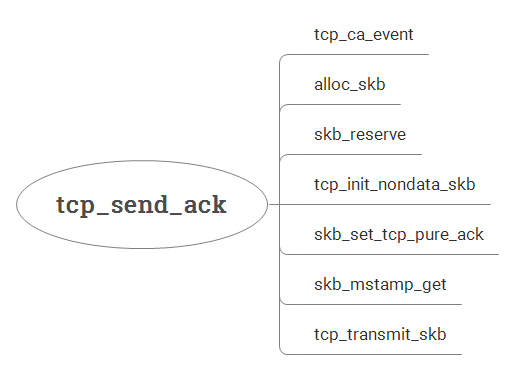
\includegraphics[width=\textwidth]  {images/Client:Send ACK.png}
                \end{figure} 
    
    \subsubsection{tcp\_send\_ack}
\label{subsubsec:tcp_send_ack}
在\ref{subsec:recv_synack}分析的代码的最后,我们看到它调用了\mintinline{c}{tcp_send_ack()}来发送ACK包,
从而实现第三次握手。

\begin{minted}[linenos]{c}
/* 
Location

    net/ipv4/tcp_output.c

Function:

    This routine sends an ack and also updates the window.

Parameter:

    sk:传输控制块
该函数用于发送ACK,并更新窗口的大小 */
void tcp_send_ack(struct sock *sk)
{
        struct sk_buff *buff;

        /* 如果当前的套接字已经被关闭了,那么直接返回。 */
        if (sk->sk_state == TCP_CLOSE)
                return;
        /*what does it using for?*/
        tcp_ca_event(sk, CA_EVENT_NON_DELAYED_ACK);

        /* We are not putting this on the write queue, so
         * tcp_transmit_skb() will set the ownership to this
         * sock.
         * 为数据包分配空间
         */
        buff = alloc_skb(MAX_TCP_HEADER, sk_gfp_atomic(sk, GFP_ATOMIC));
        if (!buff) {
                inet_csk_schedule_ack(sk);
                inet_csk(sk)->icsk_ack.ato = TCP_ATO_MIN;
                inet_csk_reset_xmit_timer(sk, ICSK_TIME_DACK,
                                          TCP_DELACK_MAX, TCP_RTO_MAX);
                return;
        }

        /* 初始化ACK包 */
        skb_reserve(buff, MAX_TCP_HEADER);
        tcp_init_nondata_skb(buff, tcp_acceptable_seq(sk), TCPHDR_ACK);

        /* We do not want pure acks influencing TCP Small Queues or fq/pacing
         * too much.
         * SKB_TRUESIZE(max(1 .. 66, MAX_TCP_HEADER)) is unfortunately ~784
         * We also avoid tcp_wfree() overhead (cache line miss accessing
         * tp->tsq_flags) by using regular sock_wfree()
         */
        skb_set_tcp_pure_ack(buff);

        /* 添加时间戳并发送ACK包 */
        skb_mstamp_get(&buff->skb_mstamp);
        tcp_transmit_skb(sk, buff, 0, sk_gfp_atomic(sk, GFP_ATOMIC));
}
\end{minted}


